\subsection{Mock-up dell'applicazione}
    \begin{flushleft}
        Qui vengono presentati i mockup relativi all'applicazione.
    \end{flushleft}
    \subsubsection{Homepage dell'applicazione}
        \begin{figure}[H]
            \centering
            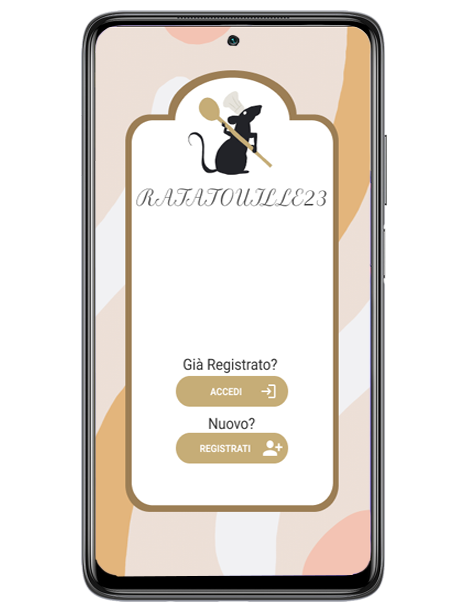
\includegraphics[width=0.70\textwidth]{assets/Mockup/Mockup_Homepage.png}
            \caption{\textbf{M01}: Homepage dell'applicazione}
            \label{fig:Mockup_Homepage}
        \end{figure}
        \begin{flushleft}
            \textbf{ID} \ \Large{\textit{\textbf{M01}}}\\
        \end{flushleft}
        \textbf{Componenti}:\\
        \begin{tabular}{lll}
            \hline
            \textbf{Tipo}   &   \textbf{Nome}   &   \textbf{Funzione} \\
            \hline
            Bottone       &   ACCEDI &   Quando cliccato porta alla schermata \textit{\textbf{M02}} \\
            \hline
            Bottone & REGISTRATI   &   Quando cliccato porta alla schermata \textit{\textbf{M03}} \\
            \hline
        \end{tabular}
        \newpage
        \subsubsection{Schermata di accesso nel sistema}
            \begin{figure}[H]
                \centering
                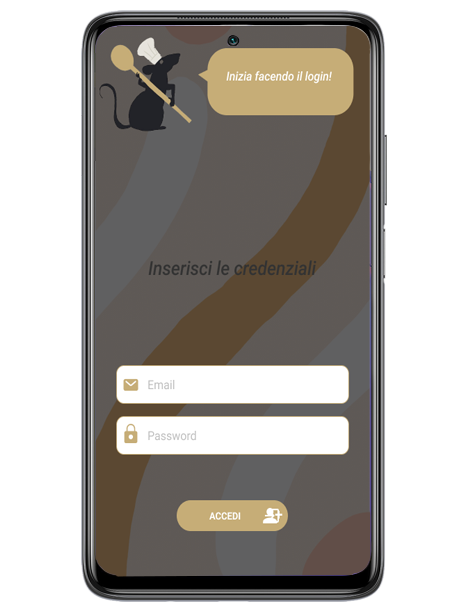
\includegraphics[width=0.70\textwidth]{assets/Mockup/Mockup_Accesso.png}
                \caption{\textbf{M02}: Schermata di accesso nel sistema}
                \label{fig:Mockup_Login}
            \end{figure}
            \begin{flushleft}
                \textbf{ID} \ \Large{\textit{\textbf{M02}}}\\
            \end{flushleft}
            \textbf{Componenti}:\\
            \begin{tabular}{lll}
                \hline
                \textbf{Tipo}   &   \textbf{Nome}   &   \textbf{Funzione} \\
                \hline
                Edit Text       &   EMAIL &   Permette l'inserimento dell'email dell'utente \\
                \hline
                Edit Text & PASSWORD  &  Permette l'inserimento della password dell'utente  \\
                \hline
                Bottone &   ENTRA   & Quando cliccato porta alla schermata \textit{\textbf{M04}} se admin, \textit{\textbf{M0?}} se dipendente \\
                \hline
            \end{tabular}
        \newpage
        \subsubsection{Schermata di registrazione nel sistema}
        \begin{figure}[H]
            \centering
            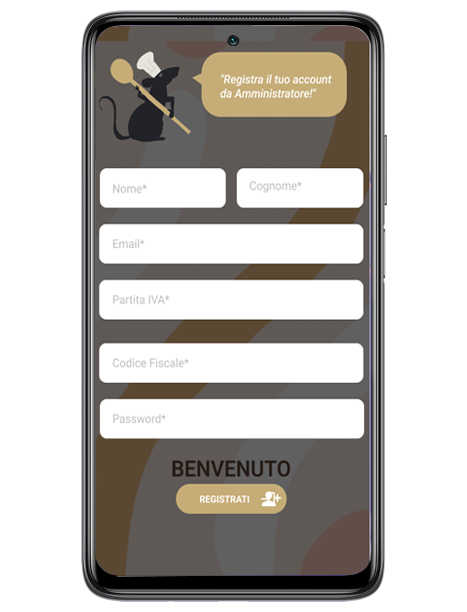
\includegraphics[width=0.60\textwidth]{assets/Mockup/Mockup_Registrazione.png}
            \caption{\textbf{M03}: Schermata di registrazione nel sistema}
            \label{fig:Mockup_Register}
        \end{figure}
        \begin{flushleft}
            \textbf{ID} \ \Large{\textit{\textbf{M03}}}\\
            \large{\textit{Nota}: la schermata di registrazione è valida solo per gli admin proprietari dei ristoranti, in quanto sono poi loro a registrare i dipendenti.}\\
        \end{flushleft}
        \textbf{Componenti}:\\
        \begin{tabular}{lll}
            \hline
            \textbf{Tipo}   &   \textbf{Nome}   &   \textbf{Funzione} \\
            \hline
            Edit Text    &   NOME    &   Permette di inserire il nome dell'admin \\
            \hline
            Edit Text & COGNOME   &  Permette di inserire il cognome dell'admin \\
            \hline
            Edit Text    &   PASSWORD    &   Permette di inserire una password per l'admin \\
            \hline
            Edit Text    &   EMAIL   &   Permette di inserire l'email dell'admin \\
            \hline
            Edit Text    & CODICE FISCALE    & Permette di inserire il codice fiscale dell'admin \\
            \hline
            Edit Text    &   P.IVA   & Permette di inserire la partita IVA dell'admin \\
            \hline
            Bottone &   REGISTRATI  & Quando cliccato riporta alla schermata \textit{\textbf{M01}} per permettere l'accesso \\
            \hline
        \end{tabular}
        \newpage
        \subsubsection{Schermata home per gli admin}
        \begin{figure}[H]
            \centering
            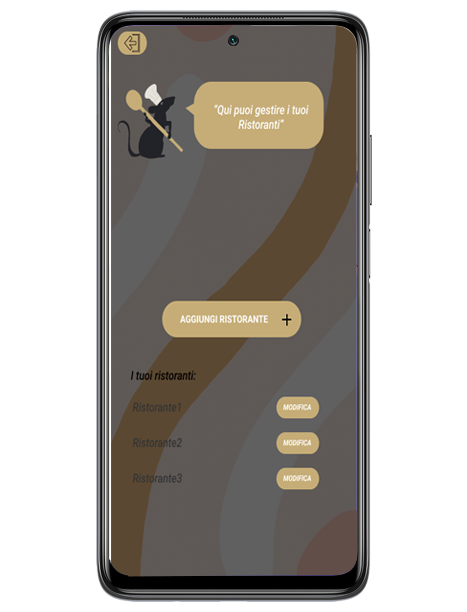
\includegraphics[width=0.70\textwidth]{assets/Mockup/Mockup_AdminDashboard.png}
            \caption{\textbf{M04}: Schermata home per gli admin}
            \label{fig:Mockup_AdminDashboard}
        \end{figure}
        \begin{flushleft}
            \textbf{ID} \ \Large{\textit{\textbf{M04}}} \\
        \end{flushleft}
        \textbf{Componenti}:\\
        \begin{tabular}{lll}
            \hline
            \textbf{Tipo}   &   \textbf{Nome}   &   \textbf{Funzione} \\
            \hline
            \multirow{2}*{ScrollView}&   \multirow{2}*{I TUOI RISTORANTI}    &   Visualizza ed eventualmente permette la modifica dei\ \ \ \ \ \ \  \\ && ristoranti registrati    \\
            \hline
            Bottone    &   AGGIUNGI RISTORANTE    &   Quando cliccato porta alla schermata \textit{\textbf{M05}} \\
            \hline
            Bottone    &   MODIFICA   &   Quando cliccato porta alla schermata \textit{\textbf{M06}} \\
            \hline
        \end{tabular}
        \newpage
        \subsubsection{Schermata di registrazione di un nuovo ristorante}
        \begin{figure}[H]
            \centering
            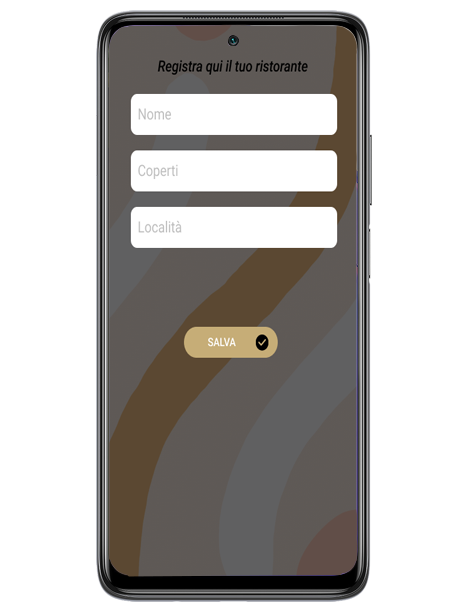
\includegraphics[width=0.65\textwidth]{assets/Mockup/Mockup_AddResturant.png}
            \caption{\textbf{M05}: Schermata di registrazione di un nuovo ristorante}
            \label{fig:Mockup_AddResturant}
        \end{figure}
        \begin{flushleft}
            \textbf{ID} \ \Large{\textit{\textbf{M05}}}
        \end{flushleft}
        \textbf{Componenti}:\\
        \begin{tabular}{lll}
            \hline
            \textbf{Tipo}   &   \textbf{Nome}   &   \textbf{Funzione} \\
            \hline
            Edit Text   &   NOME    &   Permette di inserire il nome del nuovo ristorante\\
            \hline
            Edit Text   &   LOCALITA'   &   Permette di inserire la località del nuovo ristorante\\
            \hline
            Edit Text   &   COPERTI    & Permette di inserire il n° dei coperti del nuovo ristorante\\
            \hline
            \multirow{2}*{Bottone} &   \multirow{2}*{SALVA}    &   Quando cliccato salva il nuovo ristorante nel database e torna alla schermata \\ && \textit{\textbf{M04}} \\
            \hline
        \end{tabular}
        \newpage
        \subsubsection{Schermata di modifica di un ristorante}
        \begin{figure}[H]
            \centering
            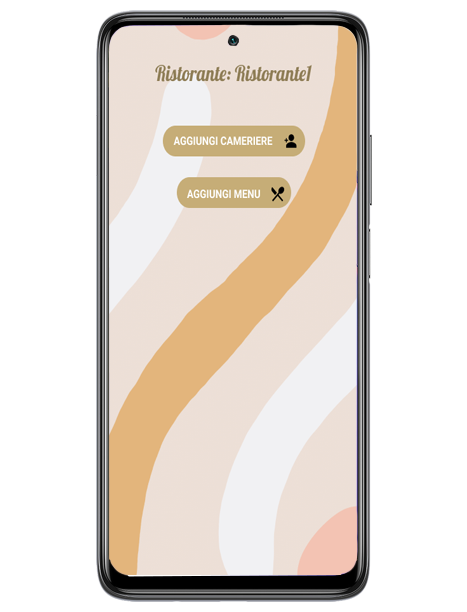
\includegraphics[width=0.70\textwidth]{assets/Mockup/Mockup_ResturantManager.png}
            \caption{\textbf{M06}: Schermata di modifica di un ristorante}
            \label{fig:Mockup_ResturantManager}
        \end{figure}
        \begin{flushleft}
            \textbf{ID} \ \Large{\textit{\textbf{M06}}}
        \end{flushleft}
        \textbf{Componenti}:\\
        \begin{tabular}{lll}
            \hline
            \textbf{Tipo}   &   \textbf{Nome}   &   \textbf{Funzione} \\
            \hline
            Bottone   &   AGGIUNGI CAMERIERE &   Quando cliccato porta alla schermata \textit{\textbf{M07}}\\
            \hline
            Bottone   &   AGGIUNGI MENU &   Quando cliccato porta alla schermata \textit{\textbf{M08}}\\
            \hline
        \end{tabular}
        \newpage
        \subsubsection{Schermata di registrazione di un nuovo dipendente}
        \begin{figure}[H]
            \centering
            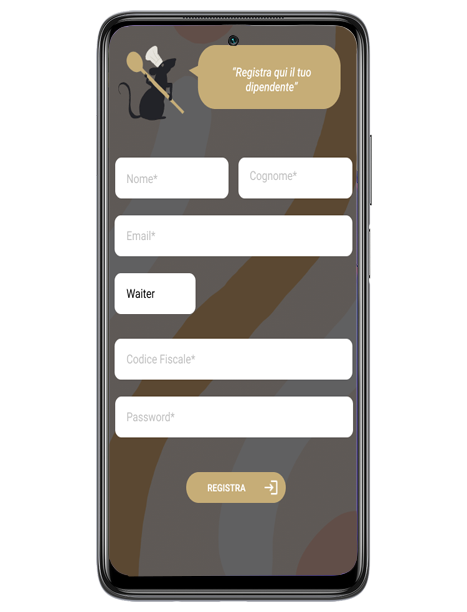
\includegraphics[width=0.60\textwidth]{assets/Mockup/Mockup_SaveWaiter.png}
            \caption{\textbf{M07}: Schermata di registrazione di un nuovo dipendente}
            \label{fig:Mockup_SaveWorker}
        \end{figure}
        \begin{flushleft}
            \textbf{ID} \ \Large{\textit{\textbf{M07}}}
        \end{flushleft}
        \textbf{Componenti}:\\
        \begin{tabular}{lll}
            \hline
            \textbf{Tipo}   &   \textbf{Nome}   &   \textbf{Funzione} \\
            \hline
            Edit Text   &   NOME    &   Permette di inserire il nome del nuovo dipendente\\
            \hline
            Edit Text   &   COGNOME   &   Permette di inserire il cognome del nuovo dipendente\\
            \hline
            \multirow{2}*{Edit Text}   &   \multirow{2}*{PASSWORD}    &   Permette di inserire la password temporanea del nuovo \\ && dipendente  \\
            \hline
            Edit Text   &   EMAIL   & Permette di inserire l'email del nuovo dipendente\\
            \hline
            Edit Text   &   CODICE FISCALE    &   Permette di inserire il codice fiscale del nuovo dipendente \\
            \hline
            \multirow{2}*{Spinner} &   \multirow{2}*{Waiter}    &   \multirow{2}*{Permette di inserire il ruolo del nuovo dipendente} \\ & (default) & \\
            \hline
            \multirow{2}*{Bottone} &   \multirow{2}*{REGISTRA}    &   Quando cliccato, se tutti i dati sono corretti, riporta alla \\ && schermata \textit{\textbf{M04}} registrando il nuovo dipendente \\
            \hline
        \end{tabular}
        \newpage
        \subsubsection{Schermata di gestione del menù}
        \begin{figure}[H]
            \centering
            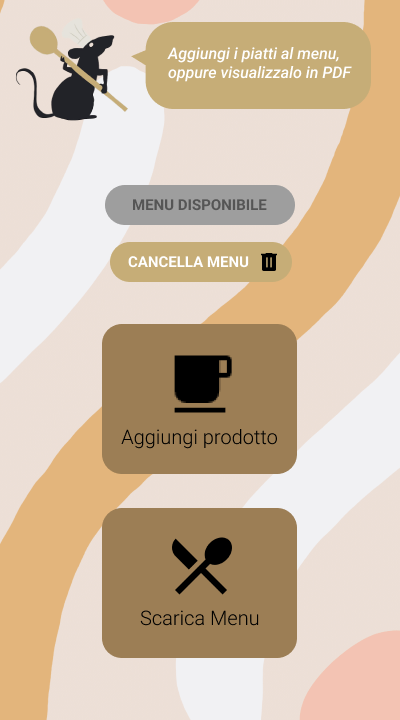
\includegraphics[width=0.70\textwidth]{assets/Mockup/Mockup_MenuManager.png}
            \caption{\textbf{M08}: Schermata di gestione del menù}
            \label{fig:Mockup_MenuManager}
        \end{figure}
        \begin{flushleft}
            \textbf{ID} \ \Large{\textit{\textbf{M08}}}
        \end{flushleft}
        \textbf{Componenti}:\\
        \begin{tabular}{lll}
            \hline
            \textbf{Tipo}   &   \textbf{Nome}   &   \textbf{Funzione} \\
            \hline
            Bottone   &   AGGIUNGI PRODOTTO    &   Quando cliccato porta alla schermata \textit{\textbf{M0?}}\\
            \hline
            \multirow{2}*{Edit Text}   &   \multirow{2}*{GENERA MENU}   &   Permette di generare il menù e salvarlo sul dispositivo in \\ && formato PDF\\
            \hline
        \end{tabular}